\documentclass[paper=a4, fontsize=11pt]{scrartcl}

\usepackage{fancyhdr}
\pagestyle{fancyplain}
\setlength{\headheight}{25pt}
\renewcommand{\headrulewidth}{0pt}
\renewcommand{\footrulewidth}{0pt}
\usepackage{graphicx}
\usepackage{epigraph}
\usepackage{amsmath,amssymb,amsfonts }
\usepackage{lastpage}
\usepackage{algorithm}
\usepackage{algpseudocode}


\newcommand{\Abf}{\ensuremath{\mathbf{A}}}
\newcommand{\bbf}{\ensuremath{\mathbf{b}}}
\newcommand{\cbf}{\ensuremath{\mathbf{c}}}
\newcommand{\abf}{\ensuremath{\mathbf{a}}}
\newcommand{\xbf}{\ensuremath{\mathbf{x}}}
\newcommand{\ybf}{\ensuremath{\mathbf{y}}}
\newcommand{\Rbb}{\ensuremath{\mathbb{R}}}
\newcommand{\Rbf}{\ensuremath{\mathbf{R}}}
\newcommand{\fo}{\ensuremath{f_0}}
\newcommand{\fii}{\ensuremath{f_i}}
\newcommand{\transpose}[1]{#1^\mathsf{T}}
\newcommand{\norm}[1]{\ensuremath{\lVert{#1}\rVert}}


\newtheorem{definition}{Definition}[section]
\newtheorem{theorem}{Theorem}[section]
\newtheorem{lemma}[theorem]{Lemma}
\newtheorem{proposition}[theorem]{Proposition}
\newtheorem{corollary}[theorem]{Corollary}
\newtheorem{observation}[theorem]{Observation}

\newenvironment{proof}[1][Proof]{\begin{trivlist}
\item[\hskip \labelsep {\bfseries #1}]}{\end{trivlist}}
%\newenvironment{definition}[1][Definition]{\begin{trivlist}
%\item[\hskip \labelsep {\bfseries #1}]}{\end{trivlist}}
\newenvironment{example}[1][Example]{\begin{trivlist}
\item[\hskip \labelsep {\bfseries #1}]}{\end{trivlist}}
\newenvironment{remark}[1][Remark]{\begin{trivlist}
\item[\hskip \labelsep {\bfseries #1}]}{\end{trivlist}}

\newcommand{\qed}{\nobreak \ifvmode \relax \else
      \ifdim\lastskip<1.5em \hskip-\lastskip
      \hskip1.5em plus0em minus0.5em \fi \nobreak
      \vrule height0.75em width0.5em depth0.25em\fi}


\newcommand{\lecture}{Assignment \#2 Report} %lecture number and date goes here
\newcommand{\lecturedate}{February 14, 2016} %lecture date goeshere
\newcommand{\scribe}{Michael Lam} %student name goes here

\fancyhead[L]{\small Winter 2016}
\fancyhead[R]{\small \lecture}
%\fancyfoot[L]{\small CS 519-006: Deep Learning}
%\fancyfoot[C]{}
\fancyfoot[C]{\thepage\ of \pageref{LastPage}}


\begin{document}


\newcommand{\horrule}[1]{\rule{\linewidth}{#1}} % Create horizontal rule command with 1 argument of height

\title{	
\normalfont \normalsize
\vspace{-30pt}
\textsc{CS 519-006: Deep Learning} \\ [10pt]
\horrule{0.5pt} \\[0.4cm] % Thin top horizontal rule
\LARGE \lecture\\ % The assignment title
\vspace{5pt}
\normalsize \scribe\\
\lecturedate\\
\horrule{2pt} \\[0.5cm] % Thick bottom horizontal rule
}


\date{} % Today's date or a custom date

\maketitle
\vspace{-100pt}
%\epigraph{''Every problem is an optimization problem in disguise.''}{--Anonymous}

\begin{abstract}
This assignment implements a one hidden layer fully connected neural network in python from scratch.  We investigate the training and testing of this network on various hyperparameters and report the results.
\end{abstract}

\section{Question 1}

{\small Write a function that evaluates the trained network (5 points), as well as computes all the subgradients of $W_1$ and $W_2$ using backpropagation (5 points).}\\

The file ``util/metrics.py'' contains functions to evaluate the trained network. It contains classes to calculate the training and test misclassification error rate (ErrorRate) and a function to use the cross entropy loss function (Objective) to calculate the training and test objective.

The subgradients of $W_1$ and $W_2$ are computed in the file ``layers/linear.py''.  The function ``gradW()'' and ``gradB()'' calculate the subgradients of the weights and biases (respectively) of the linear layer.  The backward pass can be computed using the ``backward'' function.

\section{Question 2}

{\small Write a function that performs stochastic mini-batch gradient descent training (5 points). You may use the deterministic approach of permuting the sequence of the data. Use the momentum approach described in the course slides.}\\

The stochastic mini-batch gradient descent training is implemented through the ``MomentumSolver'' class.  The parameters are updated using the stochastic mini-batch gradient descent and the ``MomentumSolver'' specifically updates the parameters using the momentum approach.

\section{Question 3}

{\small Train the network on the attached 2-class dataset extracted from CIFAR-10: (data can be found in announcement on canvas.). The data has 10,000 training examples in 3072 dimensions and 2,000 testing examples. For this assignment, just treat each dimension as uncorrelated to each other. Train on all the training examples, tune your parameters (number of hidden units, learning rate, mini-batch size, momentum) until you reach a good performance on the testing set. What accuracy can you achieve? (20 points based on the report).}\\

We found the best hyperparameters to be the following: number of hidden units set to 50, learning rate set to 0.01, momentum set to 0.6 and mini batch size set to 64. We perform greedy search to select the best hyperparameters to save time. Please see question 6 for more details.

The best testing misclassification error rate we could achieve is about 27\% before overfitting, which translates to about 73\% test accuracy.  Figure \ref{fig:overfit} shows this overfitting and test performance.  For more detailed discussion please see question 7.

\begin{figure}
\centering
\centering
 \begin{minipage}{.5\columnwidth}
\centering
  	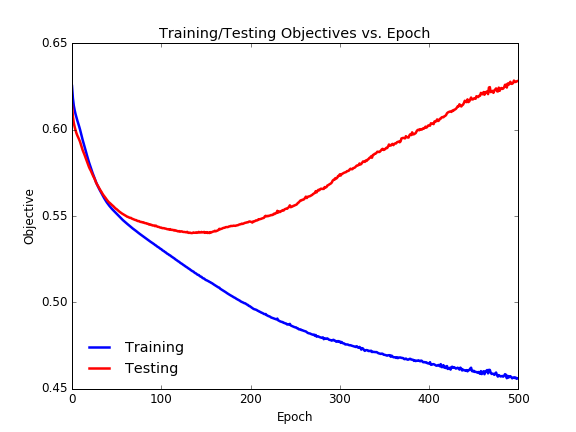
\includegraphics[width=1\linewidth]{overfit_objective.png}
  	\footnotesize{(a)}
 \end{minipage}\hfill%
\centering
 \begin{minipage}{.5\columnwidth}
\centering
  	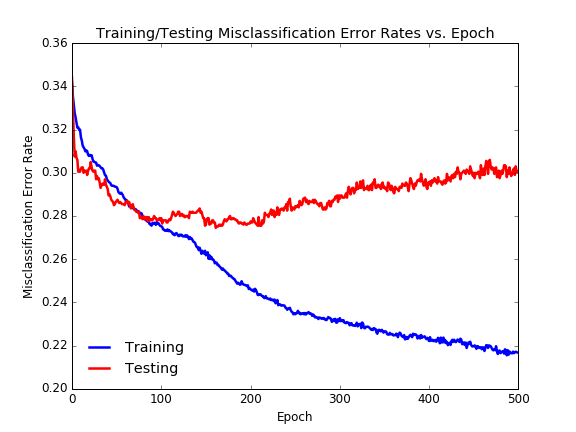
\includegraphics[width=1\columnwidth]{overfit_errorrate.png}
  	\footnotesize{(b)}
 \end{minipage}\hfill%
\caption{Overfitting phenomenon. (a) Training and testing objectives show overfitting begins around epoch 100.  (b) Training and testing misclassification error rate also shows overfitting.  We also observe a 6\% improvement on the testing set before epoch 100.}
\label{fig:overfit}
\end{figure}

\section{Question 4}

{\small Code Description: please provide detailed code description for each part of your project in the report. Every function in your code must be explained with its functionality and usage (Maximal 2 points will be deducted from each part if this is not provided).}\\

The code is commented in depth.  Each class and function should have a detailed comment explaining what it does.  The README file also gives an overview of the code.

\section{Question 5}

{\small Training Monitoring: For each epoch in training, your function should evaluate the training objective, testing objective, training misclassification error rate (error is 1 for each example if misclassifies, 0 if correct), testing misclassification error rate (5 points).}\\

The training monitoring is done through ``util/monitor.py''.  It records the training objective, testing objective, training misclassification error rate and testing misclassification error rate on each epoch into a log file.  That log file can be loaded with gnuplot, matplotlib, etc. to generate plots.  Figure \ref{fig:overfit} shows that we have the capability to monitor our training by analyzing training objective, testing objective, training misclassification error rate and testing misclassification error rate.

\section{Question 6}

{\small Tuning Parameters: please create three figures with following requirements. Save them into jpg format:
i) test accuracy with different number of batch size
ii) test accuracy with different learning rate
iii) test accuracy with different number of hidden units}\\

We experimented on the following hyperparameters: number of hidden units, learning rate, mini-batch size and momentum.  We note that after about 500 hidden units we would run out of memory or run extremely slowly (at least on the OSU HPC cluster), so we experimented on numbers below this.

Our default configuration sets the number of hidden units to 50, learning rate to 0.01, momentum to 0 and mini batch size to 256. These were chosen almost arbitrarily: we learned from lecture that mini batch size 256 seems to be standard, we set momentum to 0 so we can observe the other variables, and we set the learning rate and number of hidden units to somewhat conservative numbers.  Now when we want to investigate a certain hyperparameter, we keep the other hyperparameters fixed to this default configuration.  We could have also just exhaustively enumerated all possibilites but this would require a lot of experiments so to save time we search ``greedily'' for the best hyperparameter.

Figure \ref{fig:question6} plots the test accuracy as a function of the different number of batch sizes, learning rates and number of hidden units.

\begin{figure}
\centering
 \begin{minipage}{.5\textwidth}
 \centering
  	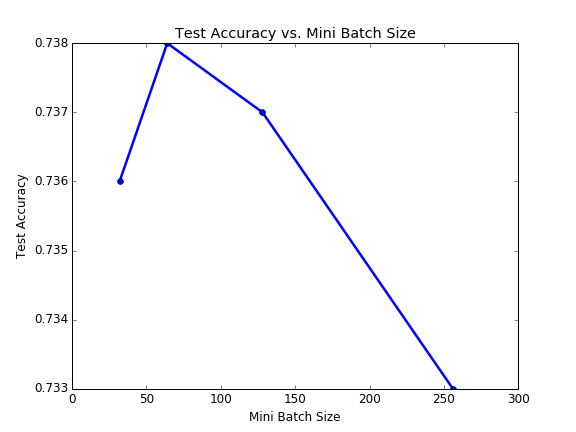
\includegraphics[width=1\linewidth]{batchsize.png}
  	\footnotesize{Mini Batch Size}
 \end{minipage}%%
 \centering
 \begin{minipage}{.5\textwidth}
 \centering
  	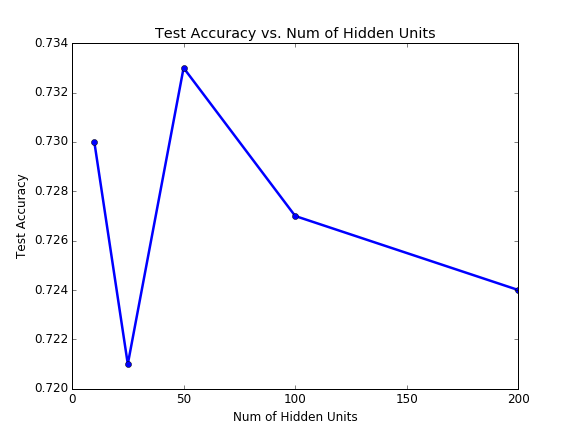
\includegraphics[width=1\linewidth]{hiddenunits.png}
  	\footnotesize{Number of Hidden Units}
 \end{minipage}
  \centering
 \begin{minipage}{.5\textwidth}
 \centering
  	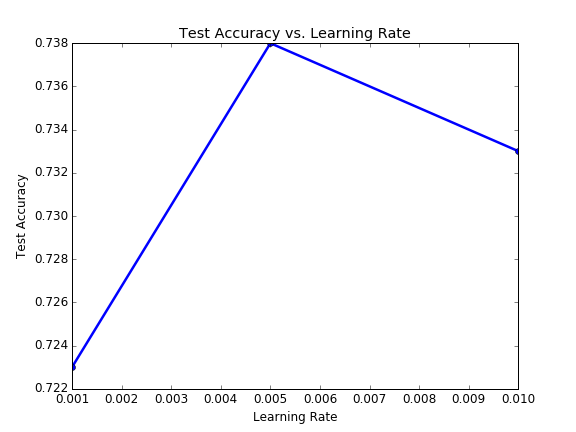
\includegraphics[width=1\linewidth]{learningrate.png}
  	\footnotesize{Learning Rate}
 \end{minipage}%%
\centering
 \begin{minipage}{.5\textwidth}
 \centering
  	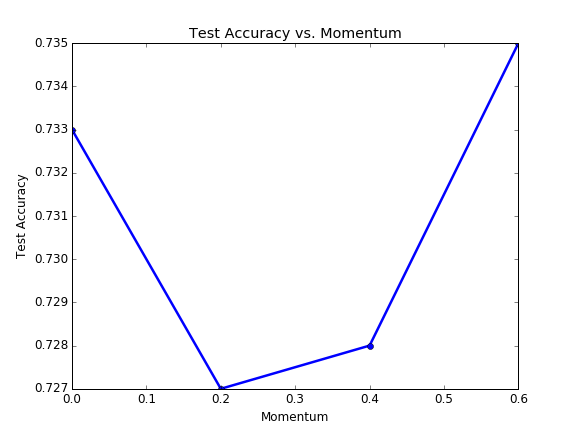
\includegraphics[width=1\linewidth]{momentum.png}
  	\footnotesize{Momentum}
 \end{minipage}
\caption{Test accuracy on various hyperparameters.}
\label{fig:question6}
\end{figure}

\section{Question 7}

{\small Discussion about the performance of your neural network.}\\

The neural network performs decently.  With the best hyperparameters so far in this report, it is able to reduce the testing misclassification error rate by about 6\% before overfitting.  We see this overfitting happening since the testing objective and testing error rate increases while the training objective and training error rate still decreases.  Overfitting occurs early, at about epoch 100.  Since the training misclassification error rate keeps reducing though, this suggests that the network was implemented correctly and learning properly.  Figure \ref{fig:overfit} demonstrates overfitting and the best performance we can obtain.

We were not satisfied with the hyperparameter tuning because some trends do not seem intuitive and we did not see much improvement.  We also did not have enough time and resources to do an exhaustive search for the best hyperparameters.  With more time and resources, we would probably be able to tune the hyperparameters better and achieve slightly better results.  Our greedy search for hyperparameters could be improved with grid search or random search.  However, we believe that a one hidden layer neural network will not be able to achieve very great accuracy anyway since it is only has one hidden layer.  Even if more hidden nodes may help, we will eventually run out of memory anyway so we will have to resort to multiple layers.  This would be good future work.

\section{Bonus}

{\small BONUS: If you make the code modular (each layer including ReLU, cross-entropy, Linear Transform to be a separate module that takes input and returns output, gradient w.r.t. input, gradient w.r.t. parameters, there are 10 bonus points which can be used to compensate for 3) as well as other assignments.}\\

The code was designed to be modular.  Layers are located in the 		``layers/'' directory and each layer implements the ``Layer'' abstract class.  Layers have a ``forward()'' function that does a forward pass for inference, ``backward()'' function that does a backward pass to compute the gradients (w.r.t. input and parameters) during backpropagation and an ``updateParams()'' function that updates the weights of the layer using momentum updates (or any other update).  One can add other layers using this API.

Loss functions are also modular.  Cross entropy is implemened through the ``Loss'' abstract class.  It has a ``forward()'' function that computes the loss and then a ``backward()'' function that computes the gradients w.r.t. the inputs, which is then used for backpropagation.  One can add other loss functions easily with this API.

The solver is also modular.  Layers that update weights use the ``updateParams()'' function, which calls solvers that implement the ``Solver'' abstract class.  Momentum solver is implemented as the ``MomentumSolver'' class.  It uses momentum updates.  One can also add other solvers with this API.

Please consult the README to learn more about the code structure and observe its modularity.

\end{document}
